\documentclass[12pt]{beamer}
\usepackage[utf8]{inputenc}
\usepackage[spanish]{babel}
\usepackage{multirow}
\usepackage{color}
\usepackage{ragged2e}

\mode<presentation>{\usetheme{CambridgeUS}}
\usecolortheme{dolphin}

\title[TASMC]{Traveler Assistant System For Mexico City TASMC}
\date{}

\begin{document}

\begin{frame}
	\begin{center}
	\begin{minipage}[t]{0.73\textwidth}	
		\begin{tabular}{ccc}
			\multirow{4}{*}{
\includegraphics[height=1.7cm]{imagenes/ipn.png}} &
			&
     	 	\multirow{4}{*}{
\includegraphics[height=1.5cm]{imagenes/escom.png}} \\
      		& Instituto Politécnico Nacional & \\
      		& Escuela Superior de Cómputo & \\
      		&&\\
		\end{tabular}
	\end{minipage}
	\end{center}
	
	\begin{center}
		\small No. de Registro: 2014-A021 \\
	\end{center}		
	
	\begin{center}
		\textcolor[RGB]{0,0,204}{\Large Traveler Assistant System For Mexico City TASMC}
	\end{center}		
		
	\begin{center}
	\begin{minipage}[t]{1\textwidth}	
		\begin{tabular}{ccc}
			Presentan & 
			\multirow{4}{*}{
\includegraphics[height=1.7cm]{imagenes/logo.png}} & Directores \\
			\scriptsize Barajas Uribe Sergio & & \scriptsize  M. en C. Macario Hernández Cruz\\
			\scriptsize Vivanco Carmona Erick Rafael & & \scriptsize M. en C. Axel Ernesto Moreno Cervantes
		\end{tabular}
	\end{minipage}
	\end{center}
\end{frame}

\section{¿Por qué TASMC?}
\begin{frame}
\frametitle{Contenido}
\tableofcontents
\end{frame}

\begin{frame}
	\frametitle{¿Por qué TASMC?}
	\begin{columns} 
		\begin{column}{5cm} 
			\begin{block}{Necesidades} \small 
				\begin{itemize}
					\item Precio y horario de vuelos
					\item Buscar un hotel
					\item Hacer un itinerario de viaje
				\end{itemize} 
			\end{block} 
		\end{column}
		\begin{column}{5cm} 
			\begin{center}
				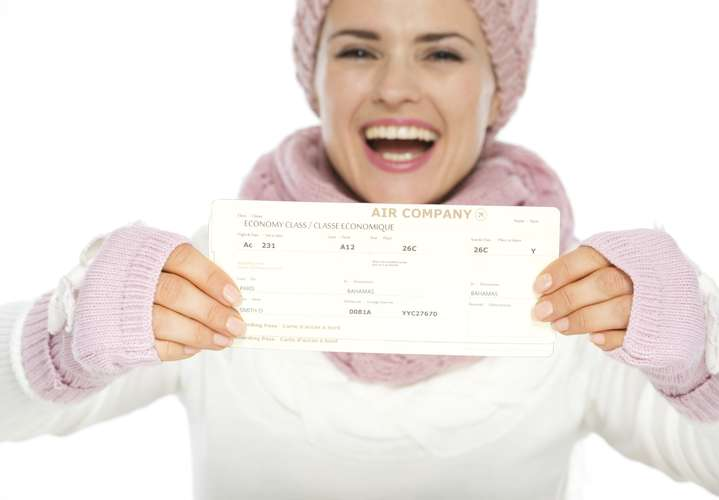
\includegraphics[height=2cm]{imagenes/nvuelo.jpg} \\
				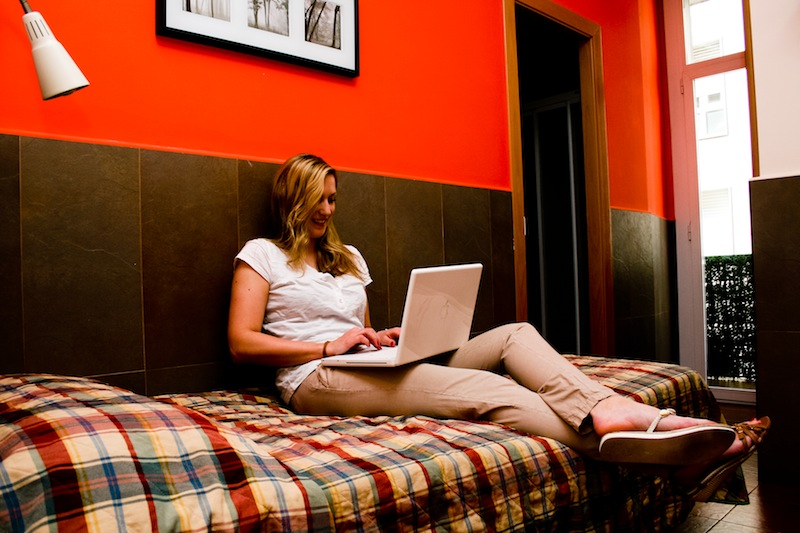
\includegraphics[height=2cm]{imagenes/nhotel.jpg} \\
				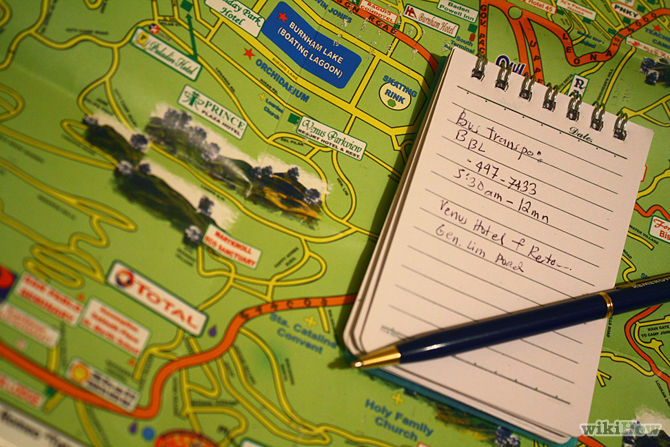
\includegraphics[height=2cm]{imagenes/nitinerario.jpg}
			\end{center} 
		\end{column} 
	\end{columns}
\end{frame}

\begin{frame}
	\frametitle{¿Por qué TASMC?}
	\begin{columns} 
		\begin{column}{5cm} 
			\begin{block}{Problemas} \small 
				\begin{itemize}
					\item Olvidar objetos 
					\item Llegar a destiempo al aeropuerto
					\item Perderse en el aeropuerto
				\end{itemize} 
			\end{block} 
		\end{column}
		\begin{column}{5cm} 
			\begin{center}
				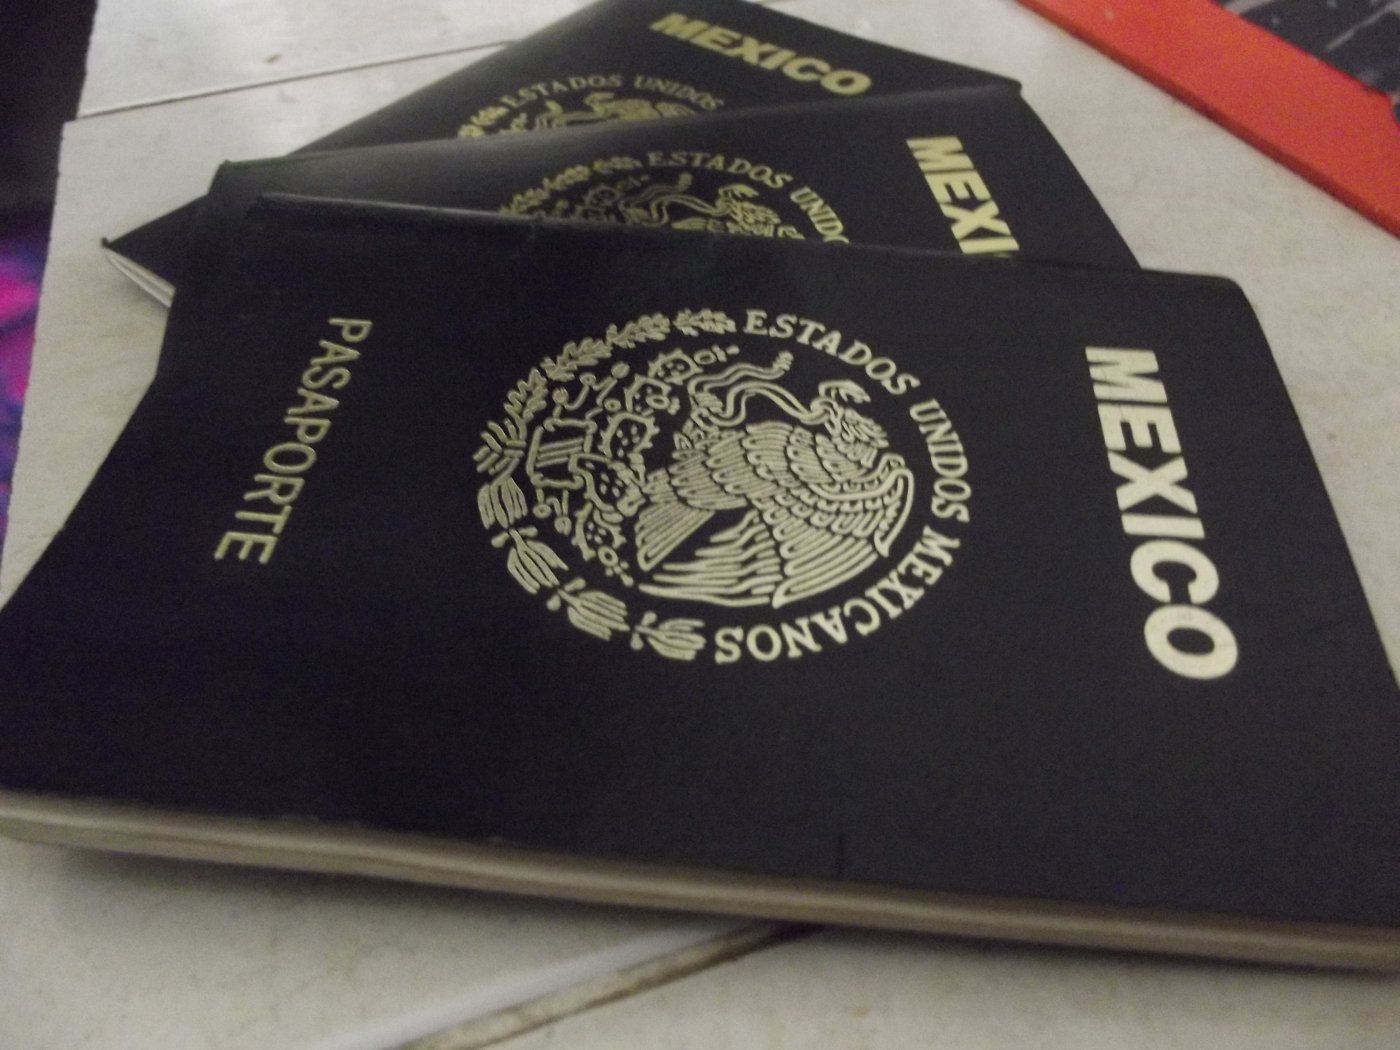
\includegraphics[height=2cm]{imagenes/pdocumento.jpg} \\
				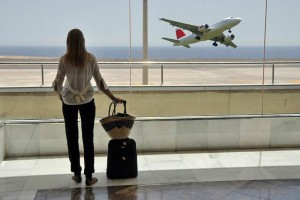
\includegraphics[height=2cm]{imagenes/pinpuntual.jpg} \\
				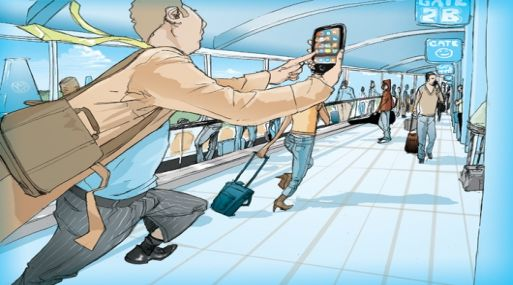
\includegraphics[height=2cm]{imagenes/pperderse.jpg}
			\end{center} 
		\end{column} 
	\end{columns}
\end{frame}

\section{¿Qué es TASMC?}
\begin{frame}[c]
	\frametitle{¿Qué es TASMC?}
	\begin{block}{}
		Sistema asistente para el viajero de la Ciudad de México
	\end{block}
	\begin{columns} 
		\begin{column}{5cm}
			\begin{block}{Características} \small 
				\begin{itemize}
					\item Configuración del viaje
					\item Vuelos disponibles
					\item Hoteles disponibles
					\item Lista de equipaje
				\end{itemize} 
			\end{block} 
		\end{column}
		\begin{column}{4cm} 
			\begin{center}
				
\includegraphics[height=5cm]{imagenes/queEs.jpg}
			\end{center} 
		\end{column} 
	\end{columns}
\end{frame}

\begin{frame}[c]
	\frametitle{¿Qué es TASMC?}
	\begin{block}{}
		Sistema asistente para el viajero de la Ciudad de México
	\end{block}
	\begin{block}{}
	 	\textbf{AICM - } Aeropuerto Internacional de la Ciudad de México
	\end{block}
	\begin{columns} 
		\begin{column}{5cm}
			\begin{block}{Características} \small 
				\begin{itemize}
					\item Itinerario de viaje
					\item Ruta al aeropuerto
					\item Ubicar dentro del AICM
					\item Información del vuelo
				\end{itemize} 
			\end{block} 
		\end{column}
		\begin{column}{4cm} 
			\begin{center}
				
\includegraphics[height=5cm]{imagenes/queEs.jpg}
			\end{center} 
		\end{column} 
	\end{columns}
\end{frame}

\section{Objetivo de TASMC}
\begin{frame}
	\frametitle{Objetivo de TASMC}
	\begin{block}{}
		\justifying
		Diseñar un sistema integral de gestión para las actividades del viajero del AICM, 
		al brindarle la información necesaria en su dispositivo móvil para hacer posible la 
		organización integral del viaje.
	\end{block}
\end{frame}

\begin{frame}
	\frametitle{Arquitectura TASMC}
	\begin{center}
		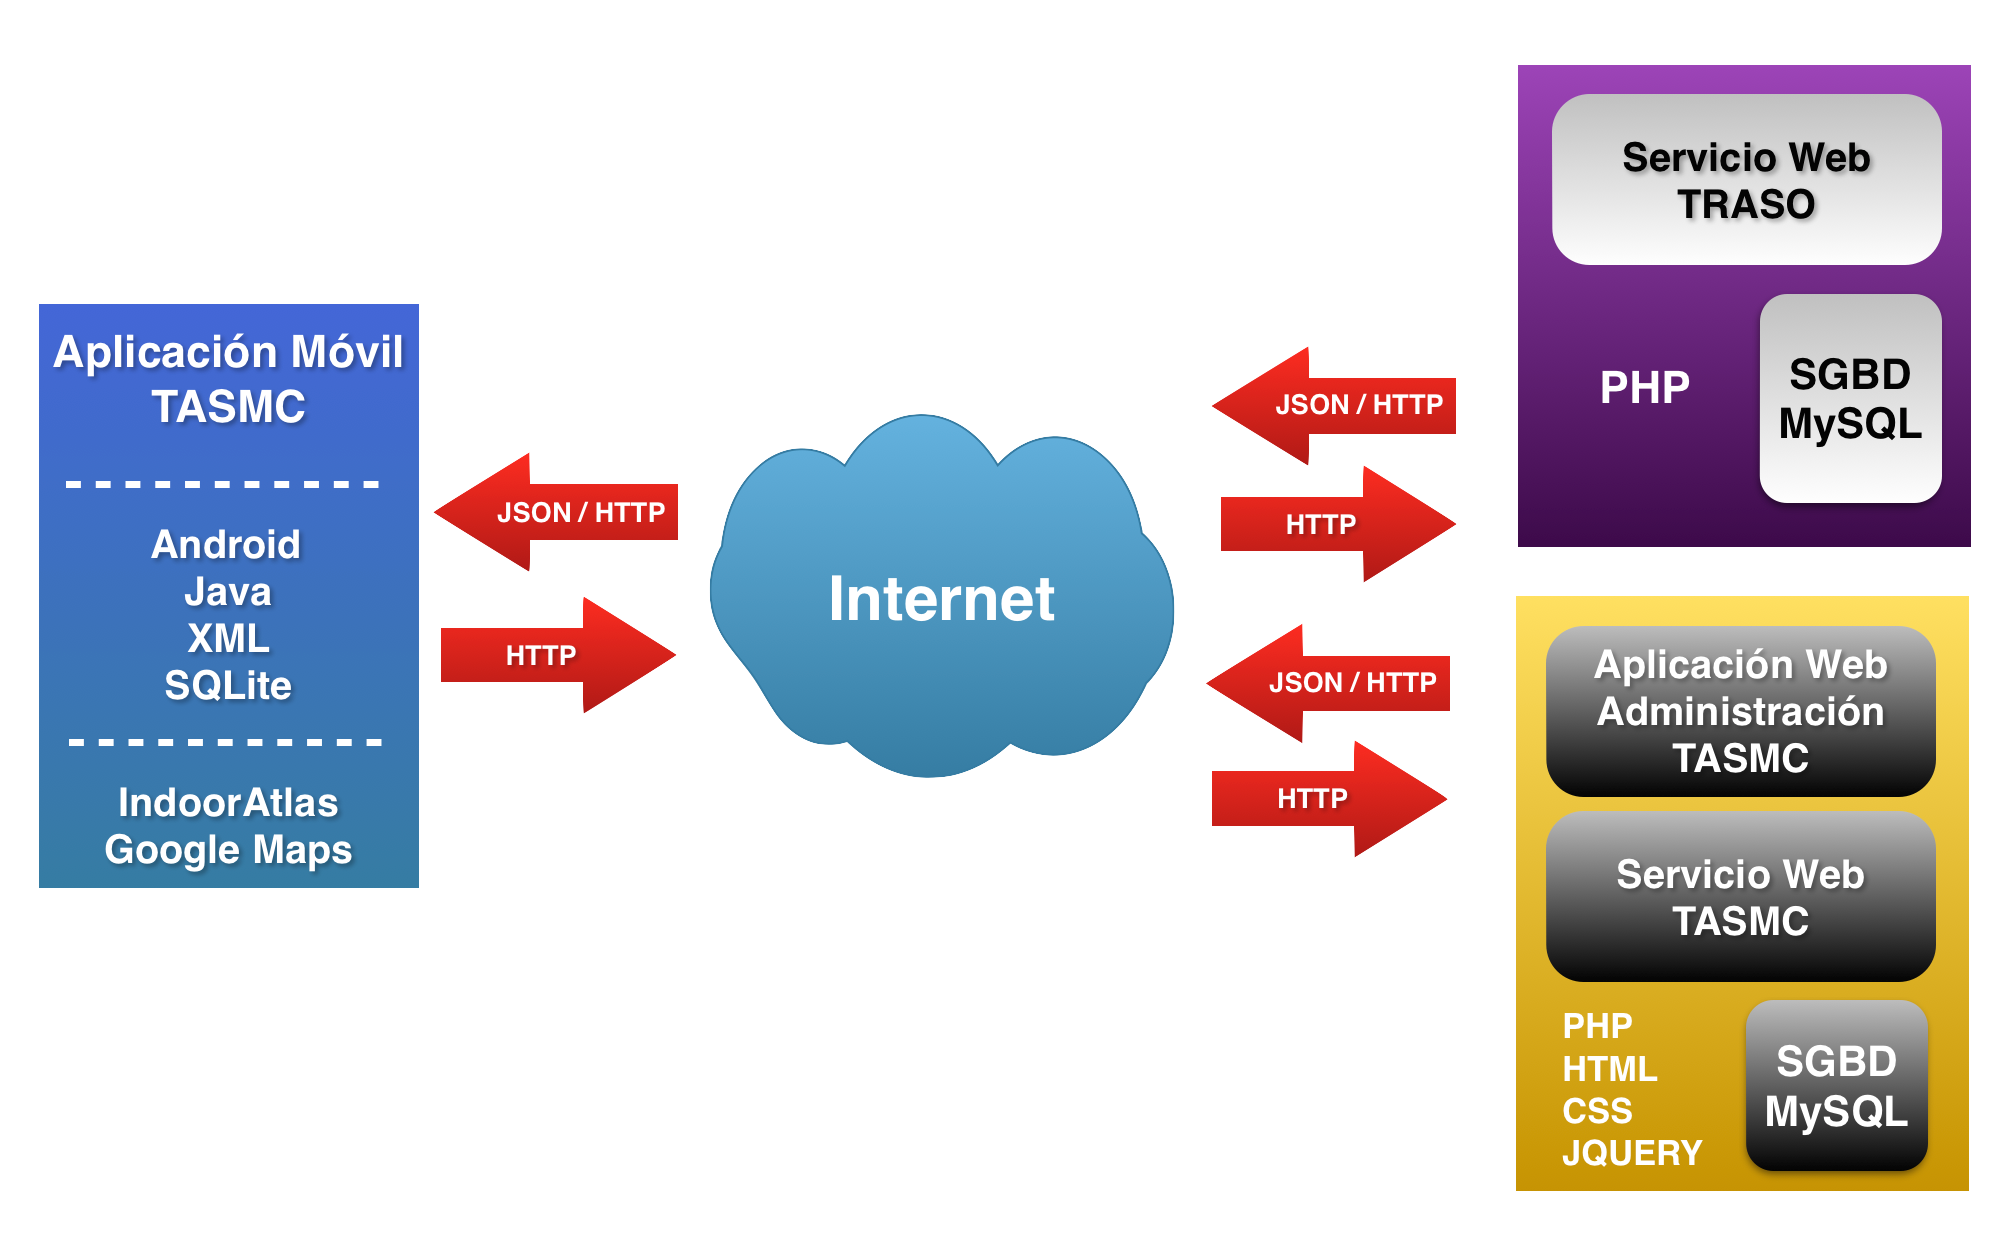
\includegraphics[height=6.5cm]{imagenes/arquitectura.png}	
	\end{center}
\end{frame}

\section{Presentación de TASMC}

\begin{frame}
	\frametitle{TASMC}
	\begin{center}
		\textcolor[RGB]{0,0,204}{\Large Traveler Assistant System For Mexico City TASMC}
	\end{center}	
	\begin{center}
		
\includegraphics[height=3.5cm]{imagenes/logo.png}
	\end{center}	
\end{frame}  

\section{Trabajo Futuro}

\begin{frame}
	\frametitle{Trabajo a Futuro}
	\begin{block}{}
		\begin{itemize}
	\item Implementar una nueva solución para la localización en interiores.
	\item Ampliar la red de información agregando los aeropuertos del mundo.
	\item Brindar el servicio de reservación dentro de TASMC.
	\item Añadir la información de todos los servicios que brinden los aeropuertos
\end{itemize}
	\end{block}

\end{frame}  

\section{Conclusiones}

\begin{frame}
	\frametitle{Conclusiones}
	\begin{block}{}
		\begin{itemize}
	\item Localización dentro del AICM.
	\item Falta de apoyo de Amadeus Web Services.
	\item El objetivo general de la aplicación queda cubierto.
\end{itemize}
	\end{block}
\end{frame}  

\begin{frame}
	\begin{center}
	\begin{minipage}[t]{0.73\textwidth}	
		\begin{tabular}{ccc}
			\multirow{4}{*}{
\includegraphics[height=1.7cm]{imagenes/ipn.png}} &
			&
     	 	\multirow{4}{*}{
\includegraphics[height=1.5cm]{imagenes/escom.png}} \\
      		& Instituto Politécnico Nacional & \\
      		& Escuela Superior de Cómputo & \\
      		&&\\
		\end{tabular}
	\end{minipage}
	\end{center}
	
	\begin{center}
		\textcolor[RGB]{0,0,204}{\Large Traveler Assistant System For Mexico City TASMC}
	\end{center}		
	
	\begin{center}
		\Large ¡Gracias por su atención!
	\end{center}
	
	\begin{columns} 
		\begin{column}{0.1cm}
			Presentan
		\end{column}
		\begin{column}{6cm} 
			Barajas Uribe Sergio

			Vivanco Carmona Erick Rafael
		\end{column} 
	\end{columns}	
	\begin{center}
		
\includegraphics[height=1.7cm]{imagenes/logo.png}
	\end{center}		
\end{frame}

\begin{frame}	
	\begin{center}
		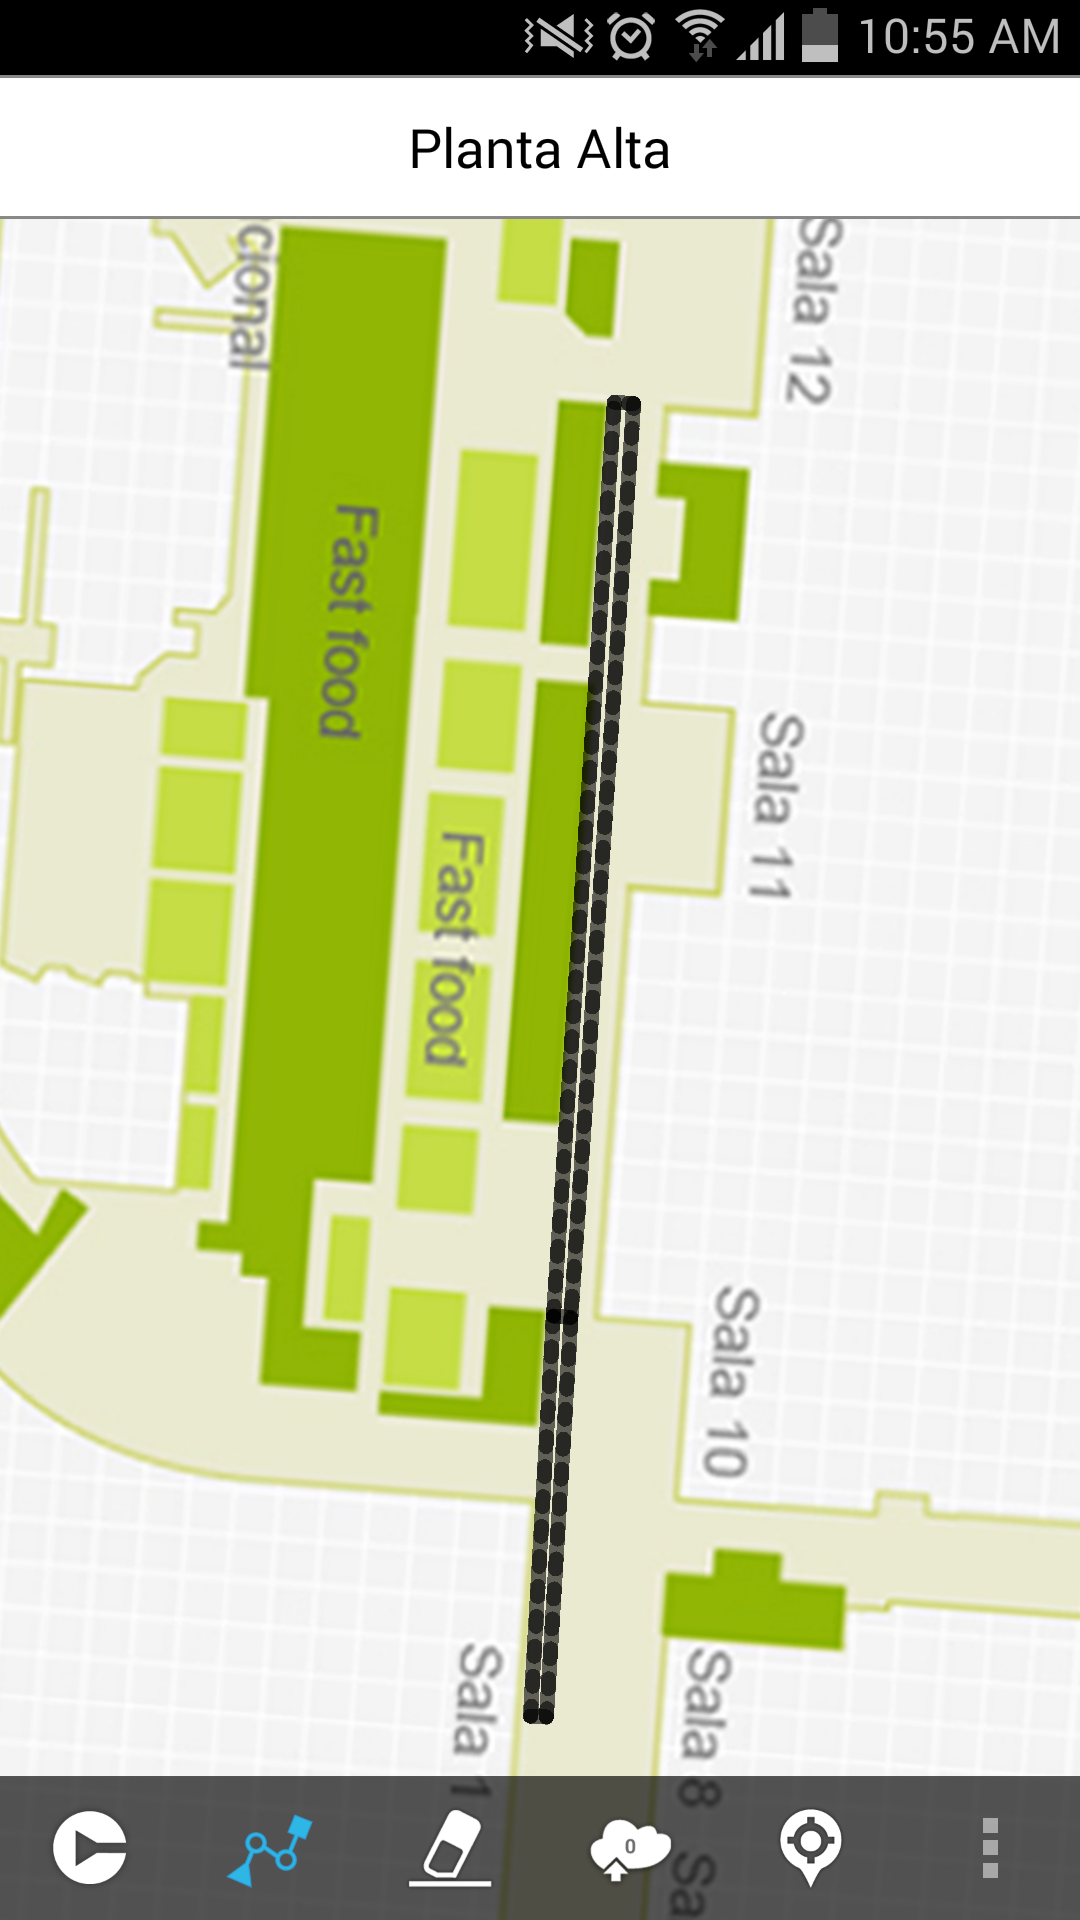
\includegraphics[height=6.5cm]{imagenes/redundante.png}
	\end{center}		
\end{frame}
	
\begin{frame}
	\frametitle{Anexo}
	\begin{center}
		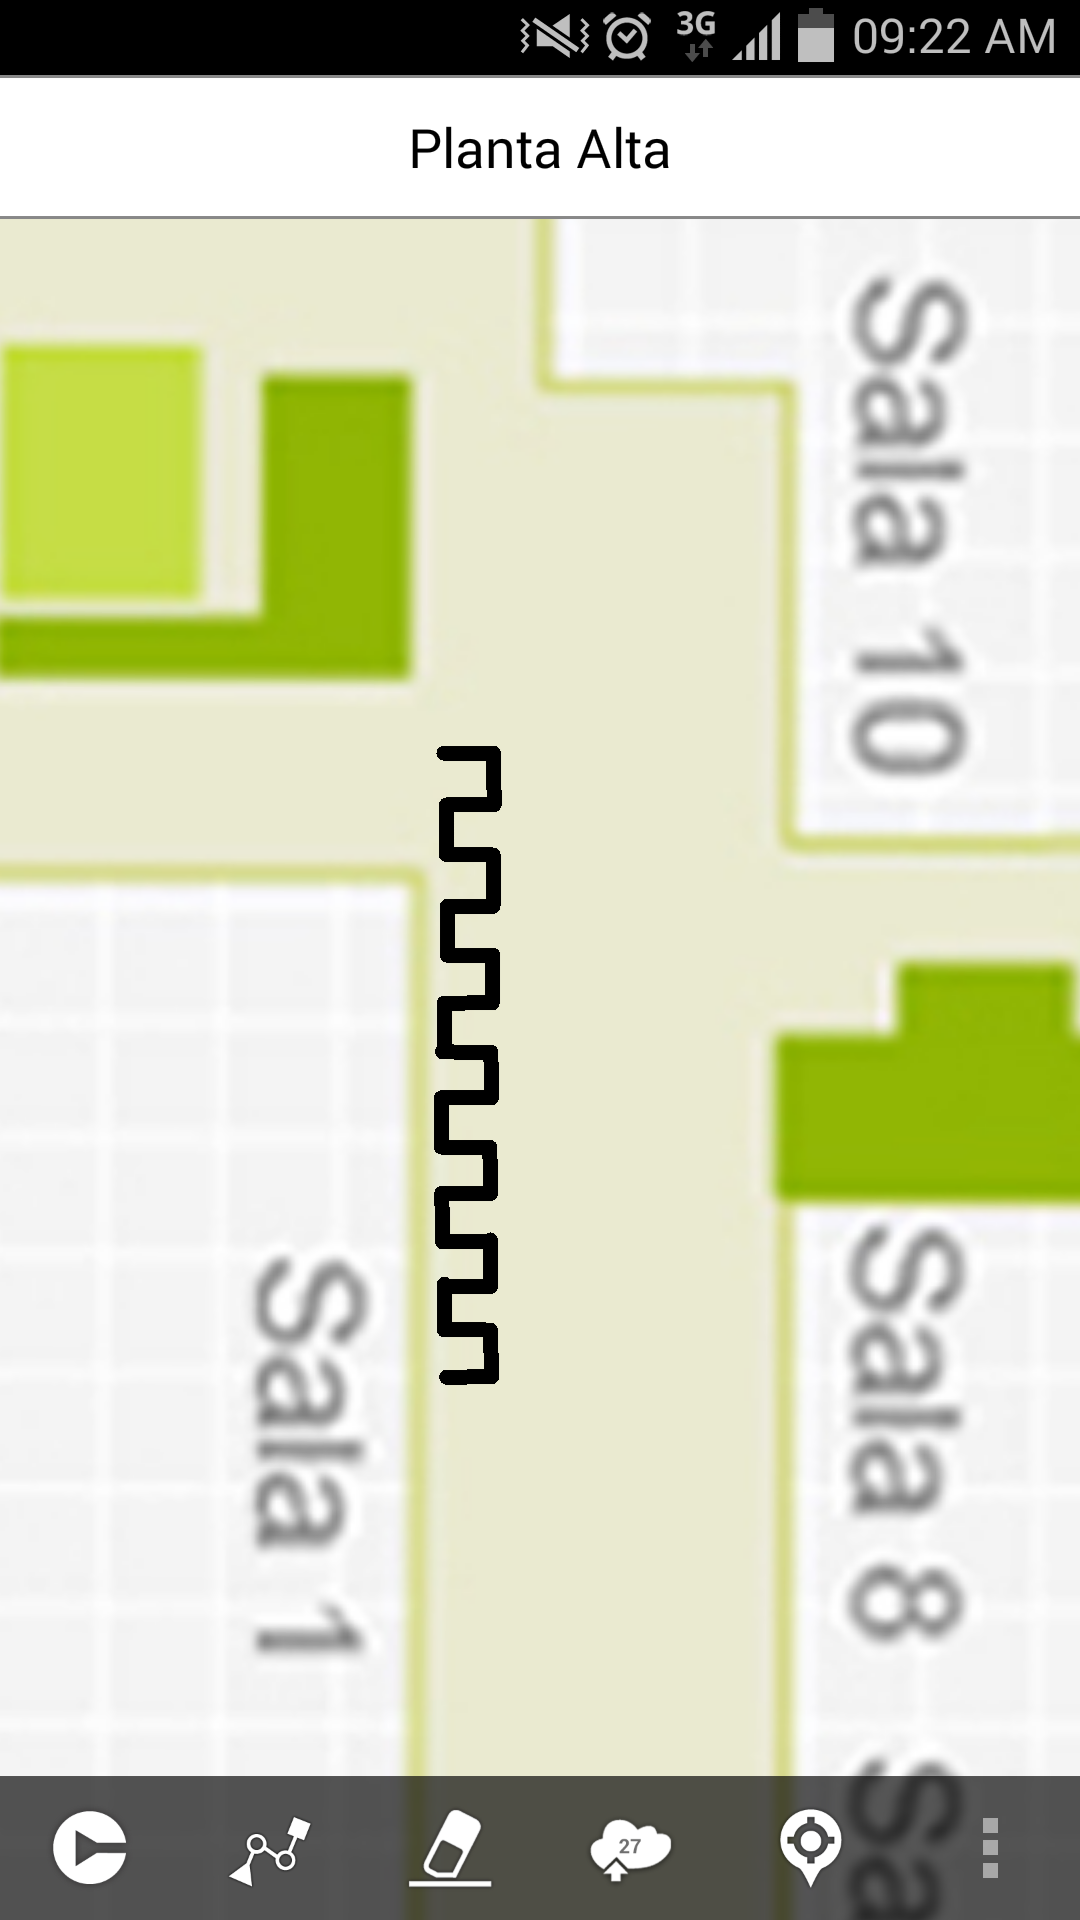
\includegraphics[height=6.5cm]{imagenes/zigzag.png}	
	\end{center}
\end{frame}

\begin{frame}
	\frametitle{Anexo}
	\begin{center}
		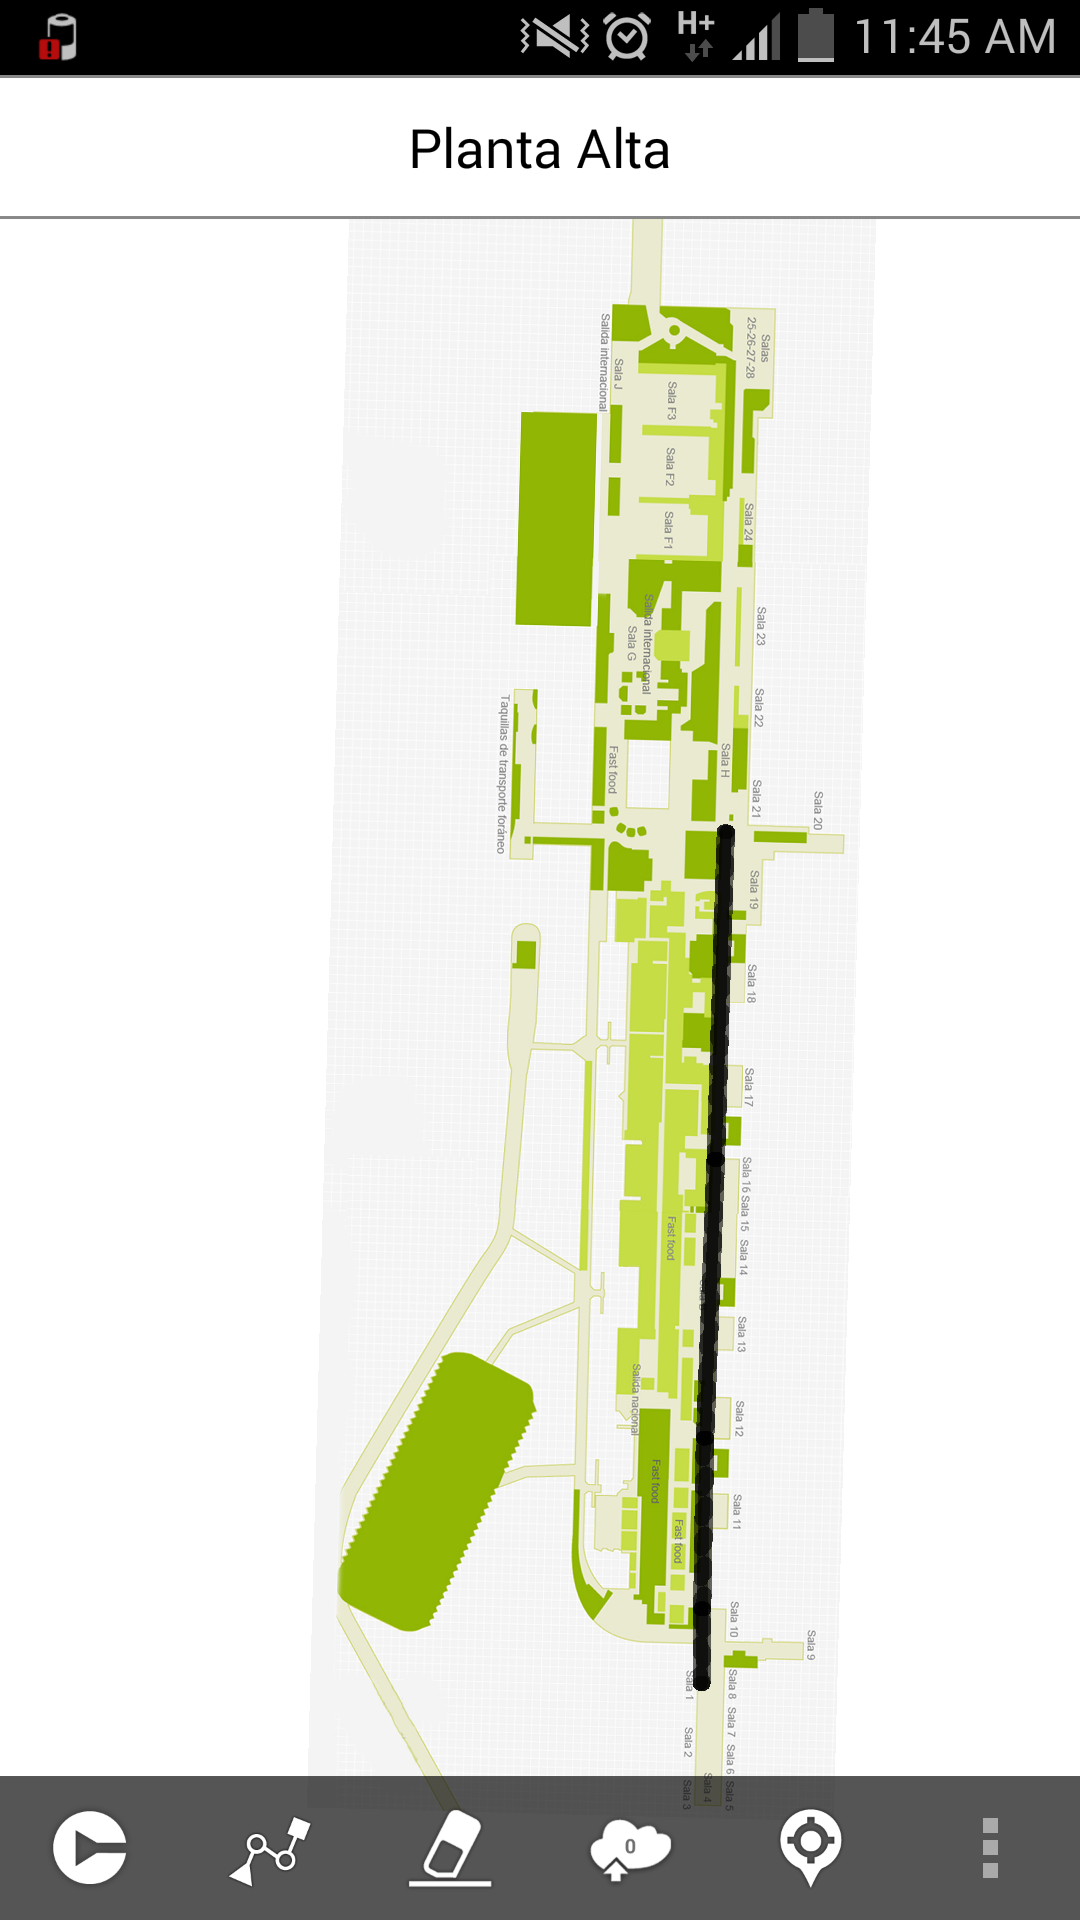
\includegraphics[height=6.5cm]{imagenes/medioback.png}	
	\end{center}
\end{frame}

\begin{frame}
	\frametitle{Anexo}
	\begin{center}
		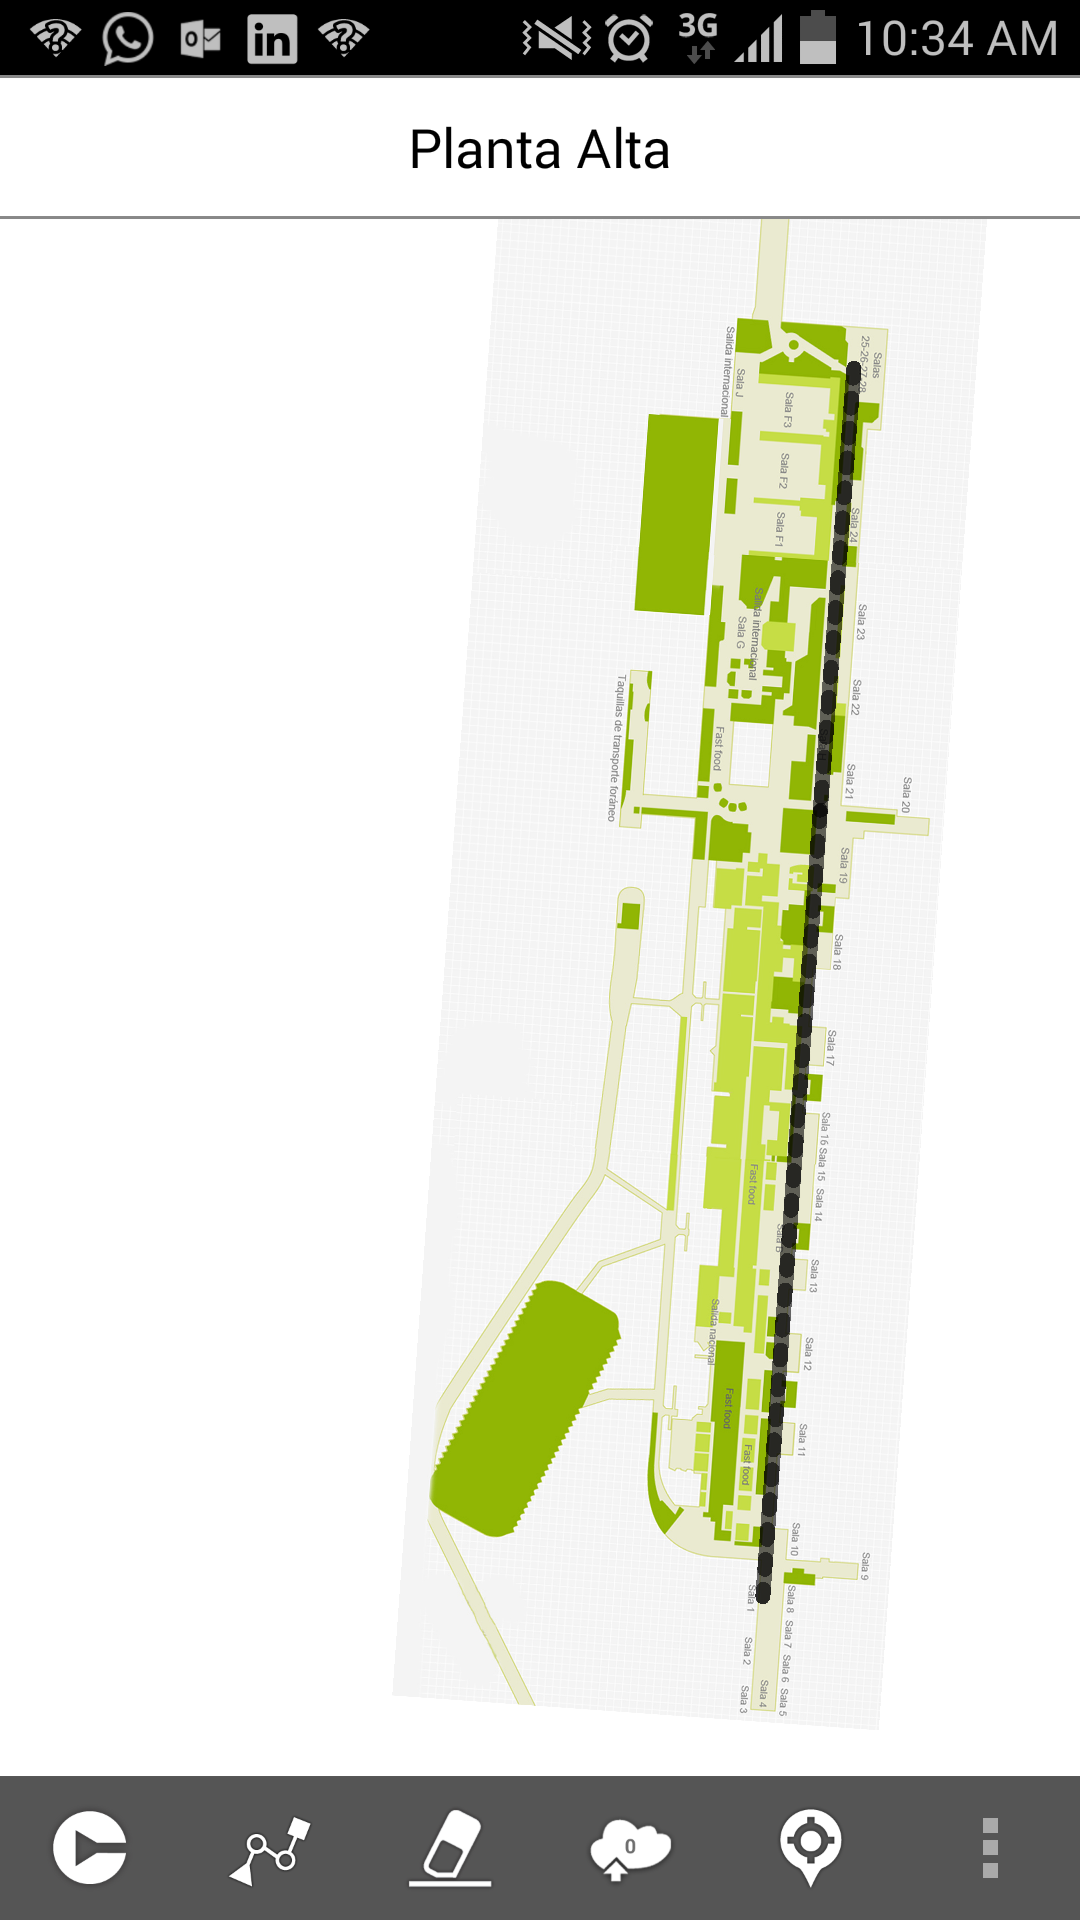
\includegraphics[height=6.5cm]{imagenes/backbone.png}	
	\end{center}
\end{frame}

\begin{frame}
	\frametitle{Anexo}
	\begin{center}
		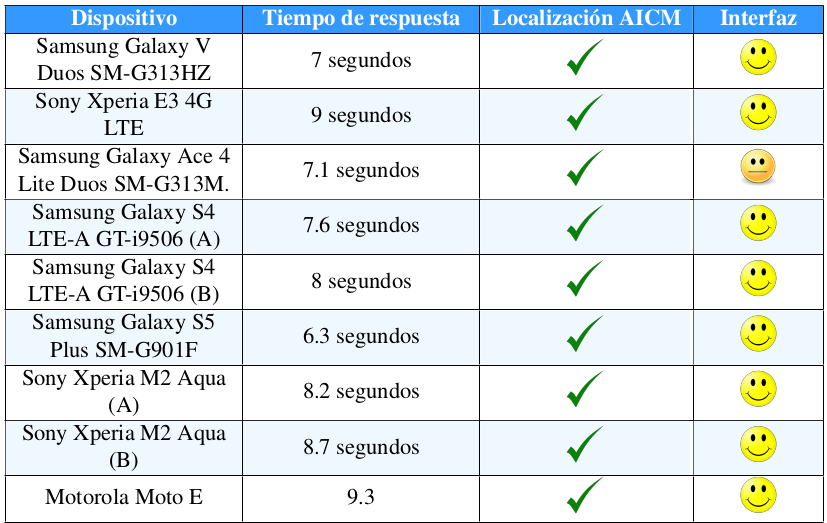
\includegraphics[height=6.5cm]{imagenes/concurrencia.png}	
	\end{center}
\end{frame}
	
\end{document}